\nwfilename{mainlitprog.nw}\nwbegindocs{0}\section{Introduction}% ===> this file was generated automatically by noweave --- better not edit it




\begin{figure}[H]
\centering
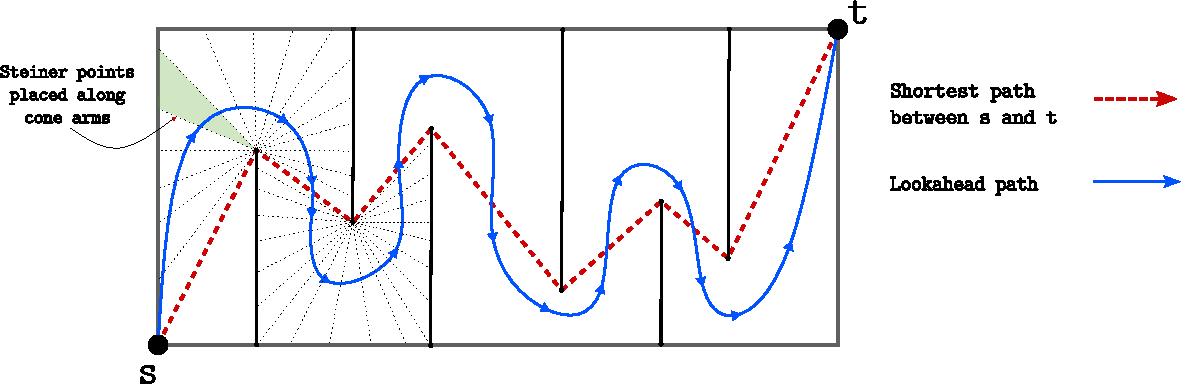
\includegraphics[width=16cm]{miscimages/stalactites-stalagmites.pdf}
\caption{Conical Routing between start $s$ and destination $t$}
\label{fig:conical-routing}
\end{figure}



This document presents a scheme  to solve the lookahead problem 
in the `stalactite and stalagmite' setting using a method based on discretizing the space into a sequence of cones. 
The hope is that, at least experimentally, this scheme will lead to short lookahead paths where each point along the 
curve can see a sufficient chunk of the curve immediately ahead of it. \footnote{We are using Euclidean visibility here
where a point $A$ sees another point $B$ iff the line segment AB is contained in the closure of the free space. }


The basic idea is captured in \autoref{fig:conical-routing}:

Since this document is meant to be a proof-of-concept, for the scheme I will 
use the following simplifying assumptions: stalactites and stalagmites 
alternate in their placement and that their arrangement is such that the shortest path between 
$s$ and $t$ is taut against their tips. 



The scheme is based on the intuition that if the string length upper bounded by a number 
\footnote{say $O(1)L$, where $L$ is the length of the shortest path between $s$ and $t$, 
          such as the red path in \autoref{fig:conical-routing}}
maximizing lookahead is equivalent to  we need to either maximizing minimum 
amount of path string in each cone (or alternatively in each line). 

Then to get the shortest path with the specified amount of lookahead we just do a binary or parametric search 
over different string lengths to find the smallest string length that does not violate the given lookahead bound. 

For the scheme 

\begin{itemize}
 \item Consider a finite sequence of small angles $\Delta \theta_i, 0 \leq i \leq N$, where $N \rightarrow \infty$,  such that 
      $\sum \Delta \theta_i =  $ reflex angle between successive segments (red segments in \autoref{fig:geomdisc}) of a shortest path incident at an 
       obstacle tip . We draw cones of angles $\Delta \theta_i, i \in \mathbb{N}$ generated by a rocking line at each stalactite and stalagmite tip 
       between these shortest path segments. In \autoref{fig:geomdisc} the area not swept by the line during its motion is a wedge facing upward (colored green).  
       Note that the green wedge itself is discretized into small cones as part of the cone sequence just mentioned. 
\item Place Steiner points separated by a small distance $\Delta x$ starting from the obstacle segment tip along each arm of every cone, for as long as the cone arm lies inside free space.
\item Draw the complete bipartite graph between the Steiner points of each cone  as shown in \autoref{fig:geomdisc}
 \item Solve the following linear program, imposing any natural shape constraints  if required.
\end{itemize}

\begin{figure}
    \centering
    \subfloat[A rocking line (blue) creates a sequence of cones of angles 
     $\Delta \theta_i$ between two successive shortest path edges]{{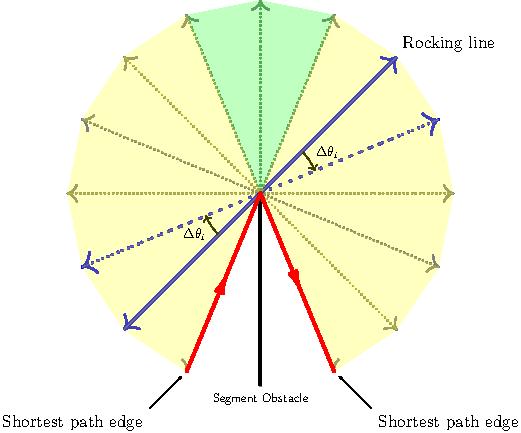
\includegraphics[width=11cm]{asy2d/rocking-line.pdf} }}
    \qquad
    \subfloat[Complete bipartite graph (green) between points on two arms of a cone on the Steiner points. 
              Distance between two consecutive Steiner points along each arm is $\Delta x$. $O$ is the tip of the 
      stalactite/stalagmite.]{{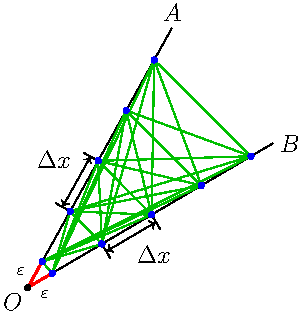
\includegraphics[width=7cm]{asy2d/bipartite-cone.pdf} }}
    \caption{Geometry of the discretization in the neighborhood of each stalactite/stalagmite tip}
    \label{fig:geomdisc}
\end{figure}

Heavy use of the CGAL kernel via its Python bindings have been made in the code which implements the scheme above to ensure
all geometric computations are precise. 

\nwenddocs{}


